\documentclass[11pt,a4paper]{article}
\usepackage[utf8]{inputenc}
\usepackage[T1]{fontenc}
\usepackage{geometry}
\usepackage{graphicx}
\usepackage{float}
\usepackage{hyperref}
\usepackage{xcolor}
\usepackage{enumitem}
\usepackage{titlesec}
\usepackage{setspace}
\usepackage{parskip}

\geometry{margin=1in}
\setstretch{1.1}
\hypersetup{
    colorlinks=true,
    linkcolor=blue,
    urlcolor=blue
}

\titleformat{\section}{\Large\bfseries}{}{0em}{}
\titleformat{\subsection}{\large\bfseries}{}{0em}{}

\title{\textbf{Sax Performance Booking Platform}\\Product Documentation}
\author{Prepared for Product Planning and MVP Delivery}
\date{\today}

\begin{document}
\maketitle
\tableofcontents
\newpage

\section{Product Overview}

\subsection{Core Idea}
This platform connects two groups in one focused marketplace:
\begin{itemize}[leftmargin=1.5em]
    \item Event organizers who need reliable live saxophone performers.
    \item Saxophonists who want consistent, visible access to paid gigs.
\end{itemize}

In simple terms: \textbf{``Uber for live sax performances.''}

\subsection{Problem Statement}
The current booking flow is fragmented and mostly informal:
\begin{itemize}[leftmargin=1.5em]
    \item Word-of-mouth referrals
    \item WhatsApp groups and private contacts
    \item Last-minute uncertainty around quality and availability
\end{itemize}

This creates friction for both demand and supply. The platform solves this by adding:
\begin{itemize}[leftmargin=1.5em]
    \item \textbf{Structure}: standardized profiles and booking workflows
    \item \textbf{Visibility}: discoverable talent with searchable filters
    \item \textbf{Trust}: ratings, reviews, and eventual verification
\end{itemize}

\section{Target Users}

\subsection{Event Organizers}
\begin{itemize}[leftmargin=1.5em]
    \item Wedding and birthday planners
    \item Church and community event organizers
    \item Corporate and private event hosts
\end{itemize}

\subsection{Saxophonists}
\begin{itemize}[leftmargin=1.5em]
    \item Professional performers
    \item Semi-professional musicians with strong stage presence
    \item Emerging talent seeking recurring bookings
\end{itemize}

\section{MVP Features (Version 1)}

\subsection{1) Saxophonist Profiles}
Each saxophonist profile should include:
\begin{itemize}[leftmargin=1.5em]
    \item Profile photo
    \item Short bio
    \item Location
    \item Price range
    \item Performance videos
    \item Ratings and reviews
\end{itemize}

\textbf{Critical rule:} no performance video significantly reduces trust and conversion.

\subsection{2) Booking System}
Booking flow should support:
\begin{itemize}[leftmargin=1.5em]
    \item Date selection
    \item Event type selection (wedding, birthday, church, etc.)
    \item Duration options (1 hour, 2 hours, full event)
    \item Request booking and instant booking modes
\end{itemize}

\subsection{3) Location-Based Discovery}
Search and discovery requirements:
\begin{itemize}[leftmargin=1.5em]
    \item ``Saxophonists near me''
    \item Filter by city
    \item Filter by price
    \item Filter by rating
\end{itemize}

\subsection{4) In-App Messaging}
Messaging should allow organizer and performer to:
\begin{itemize}[leftmargin=1.5em]
    \item Clarify event details
    \item Negotiate scope and expectations
    \item Build confidence before final booking
\end{itemize}

\subsection{5) Payments (Post-MVP Upgrade)}
Planned payment capabilities:
\begin{itemize}[leftmargin=1.5em]
    \item Partial deposits
    \item Full payment support
    \item Automatic platform commission handling
\end{itemize}

\section{Differentiating Product Features}

\subsection{Live Performance Feed}
A short-form performance feed (similar to Reels/TikTok) where saxophonists post clips.
This improves discovery quality and can accelerate organic growth.

\subsection{AI-Powered Suggestions}
Future recommendation engine:
\begin{itemize}[leftmargin=1.5em]
    \item Match organizer budget and event vibe
    \item Suggest top-fit saxophonists automatically
\end{itemize}

\subsection{Verification System}
Verified badges based on:
\begin{itemize}[leftmargin=1.5em]
    \item Identity checks
    \item Performance quality checks
\end{itemize}

\subsection{Event Matching Board}
Organizer posts a request (e.g., date + budget + event type), then saxophonists apply.

\section{Business and Monetization Model}
\begin{itemize}[leftmargin=1.5em]
    \item \textbf{Commission per booking}: 10--20\%
    \item \textbf{Premium performer profiles}: boosted visibility
    \item \textbf{Featured listings}: paid discovery slots
    \item \textbf{Subscriptions for saxophonists}: advanced profile and analytics tools
\end{itemize}

\section{Technology Stack}
\begin{itemize}[leftmargin=1.5em]
    \item \textbf{Frontend}: Flutter (mobile-first)
    \item \textbf{Backend}: Supabase (Auth, Database, Realtime)
    \item \textbf{Media Storage}: Supabase Storage or Cloudinary
    \item \textbf{Maps}: Google Maps API
    \item \textbf{Payments}: Paystack / Flutterwave
\end{itemize}

\section{Design Direction}
The visual direction follows \textbf{The Midnight Virtuoso} design system:
\begin{itemize}[leftmargin=1.5em]
    \item Dark, premium atmosphere with gold accents
    \item Editorial spacing and typography hierarchy
    \item Tonal layering over hard borders
    \item High trust through clean media-first profile presentation
\end{itemize}

\section{Challenges and Risk Areas}
\begin{itemize}[leftmargin=1.5em]
    \item Cold-start challenge: balancing initial organizer and saxophonist supply
    \item Trust barrier: users are cautious about paying unfamiliar performers
    \item Price inconsistency among performers
    \item Data and connectivity constraints for video-heavy experiences
\end{itemize}

\section{Execution Strategy}

\subsection{MVP Rollout (Do Not Overbuild)}
Start with:
\begin{itemize}[leftmargin=1.5em]
    \item Saxophonist sign-up and profile creation
    \item Basic search and filtering
    \item Booking request workflow (no integrated payment yet)
    \item In-app chat
\end{itemize}

\subsection{Growth Strategy}
Leverage creator advantage and existing audience:
\begin{itemize}[leftmargin=1.5em]
    \item Personally recruit quality saxophonists
    \item Capture high-quality performance videos
    \item Drive content distribution via TikTok and short-form channels
    \item Activate existing audience/community channels
\end{itemize}

\section{Product Naming Options}
\begin{itemize}[leftmargin=1.5em]
    \item SaxLink
    \item SaxConnect
    \item BookASax
    \item SaxHub
    \item GigSax
    \item Saxify
\end{itemize}

\section{Interface Screens (Current Assets)}

\subsection{App Launch and Role Selection}
\begin{figure}[H]
    \centering
    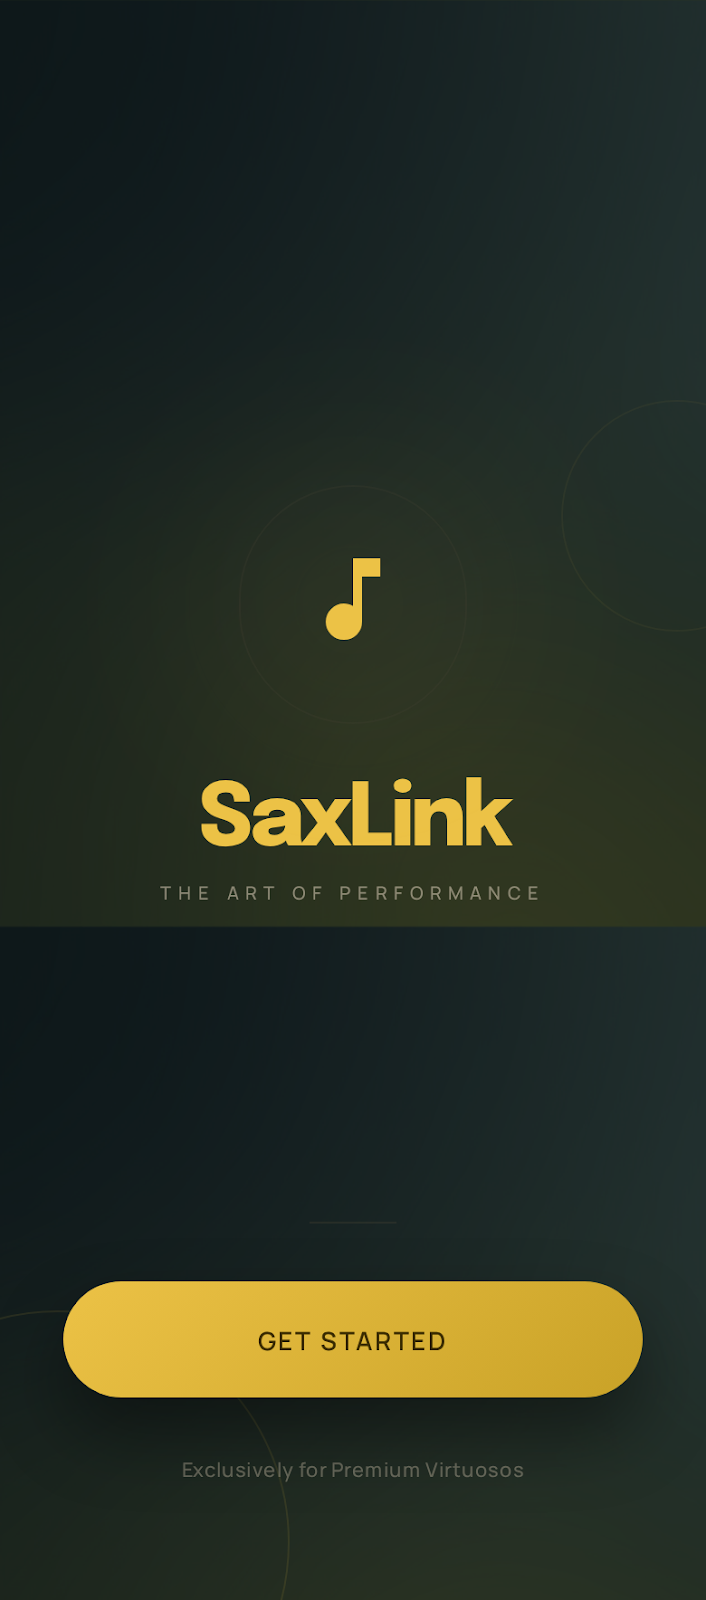
\includegraphics[width=0.44\textwidth]{splash.png}\hfill
    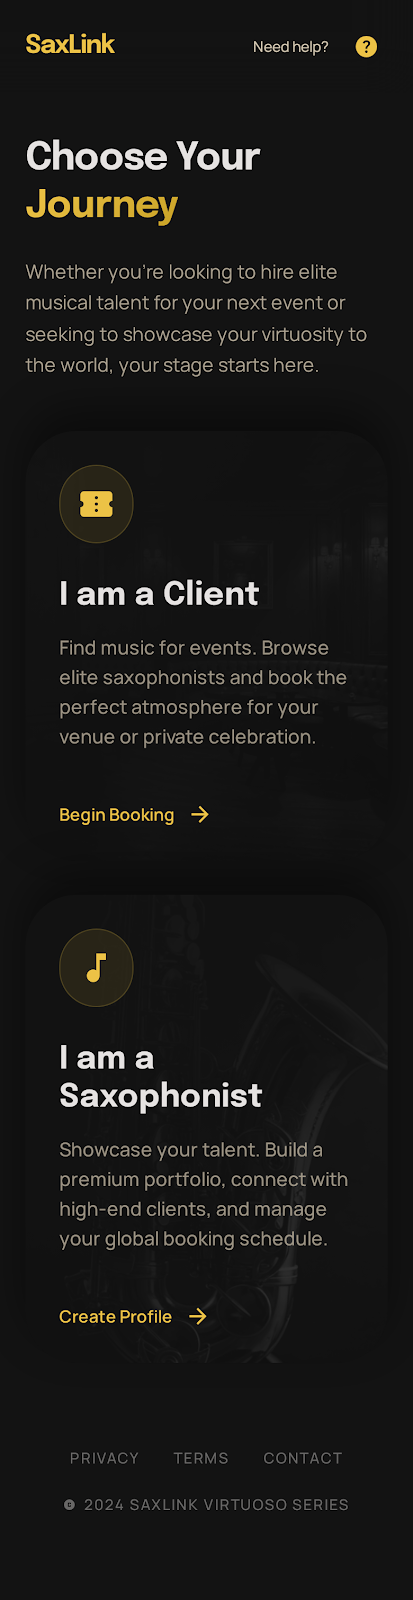
\includegraphics[width=0.44\textwidth]{role_selection.png}
    \caption{Splash screen and role selection screen}
\end{figure}

\subsection{Organizer Discovery and Booking}
\begin{figure}[H]
    \centering
    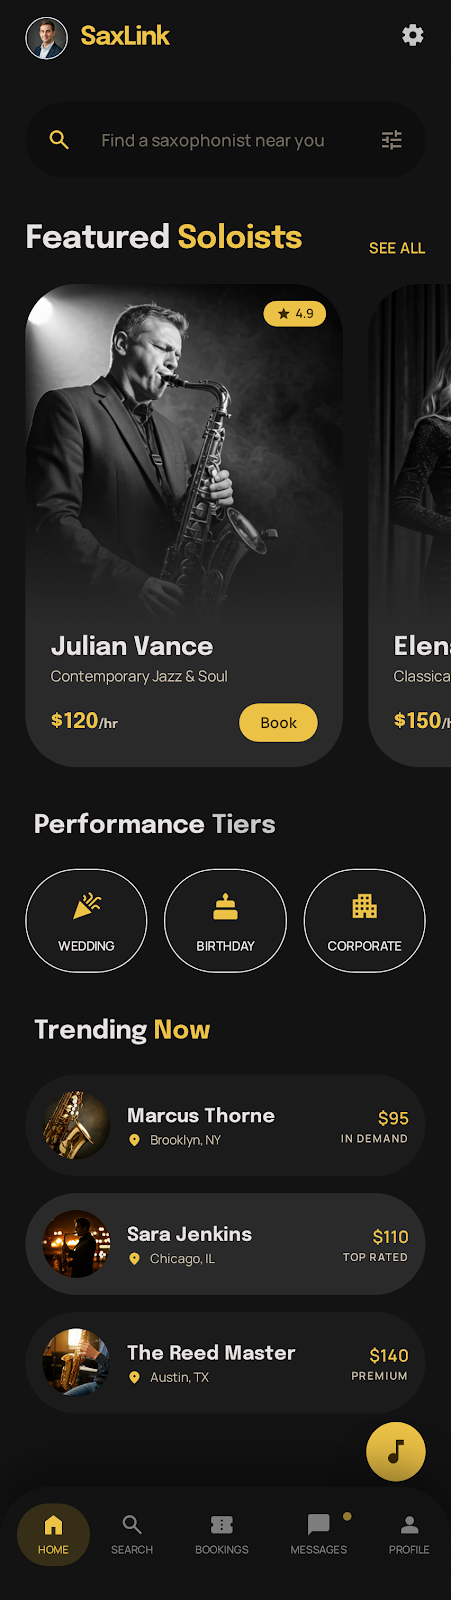
\includegraphics[width=0.44\textwidth]{client_home.png}\hfill
    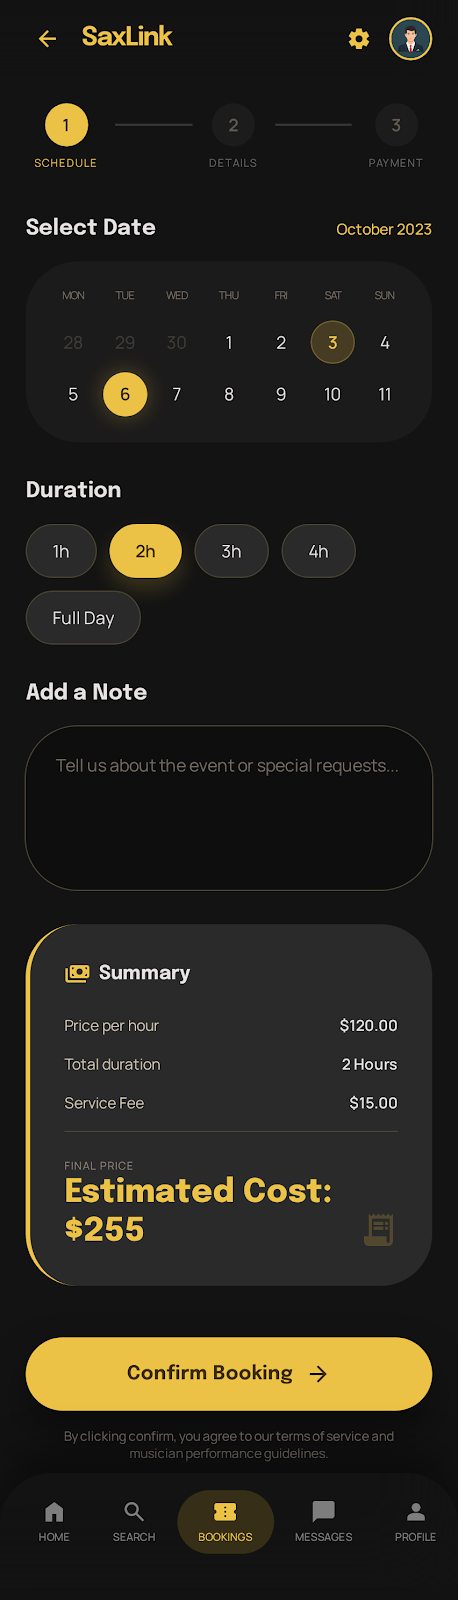
\includegraphics[width=0.44\textwidth]{booking.png}
    \caption{Organizer home and booking flow}
\end{figure}

\subsection{Saxophonist Experience}
\begin{figure}[H]
    \centering
    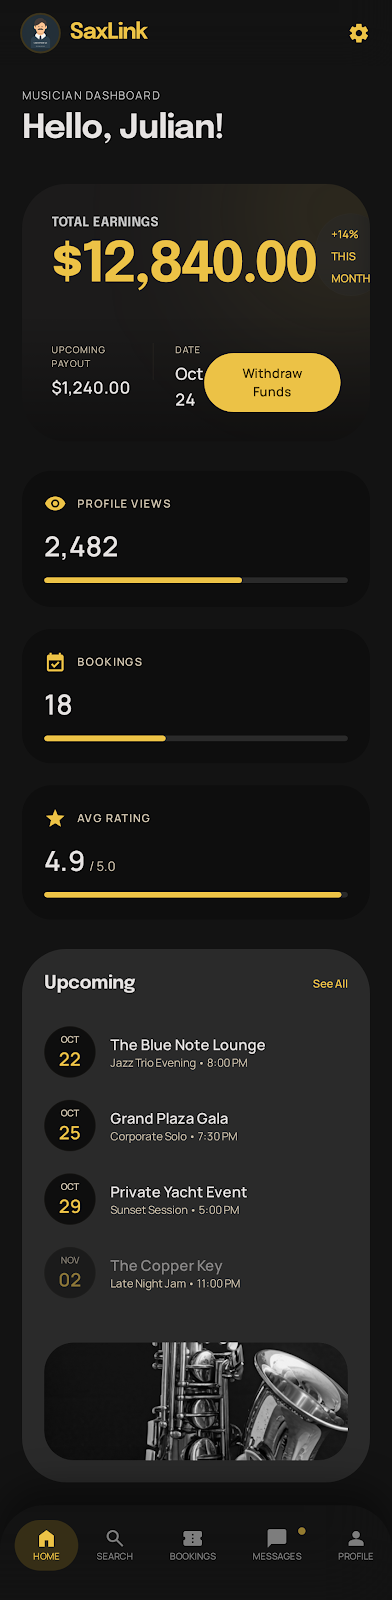
\includegraphics[width=0.44\textwidth]{dashboard.png}\hfill
    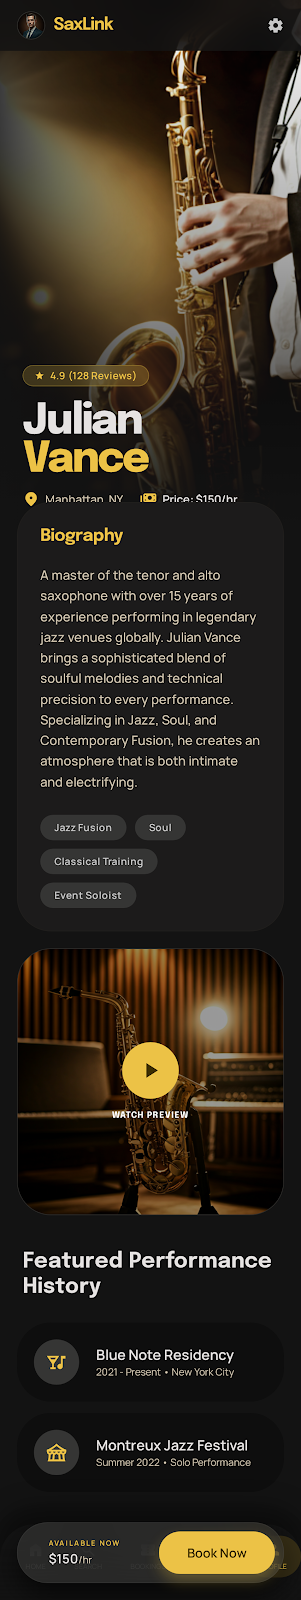
\includegraphics[width=0.44\textwidth]{profile.png}
    \caption{Saxophonist dashboard and profile}
\end{figure}

\subsection{Engagement and Performance}
\begin{figure}[H]
    \centering
    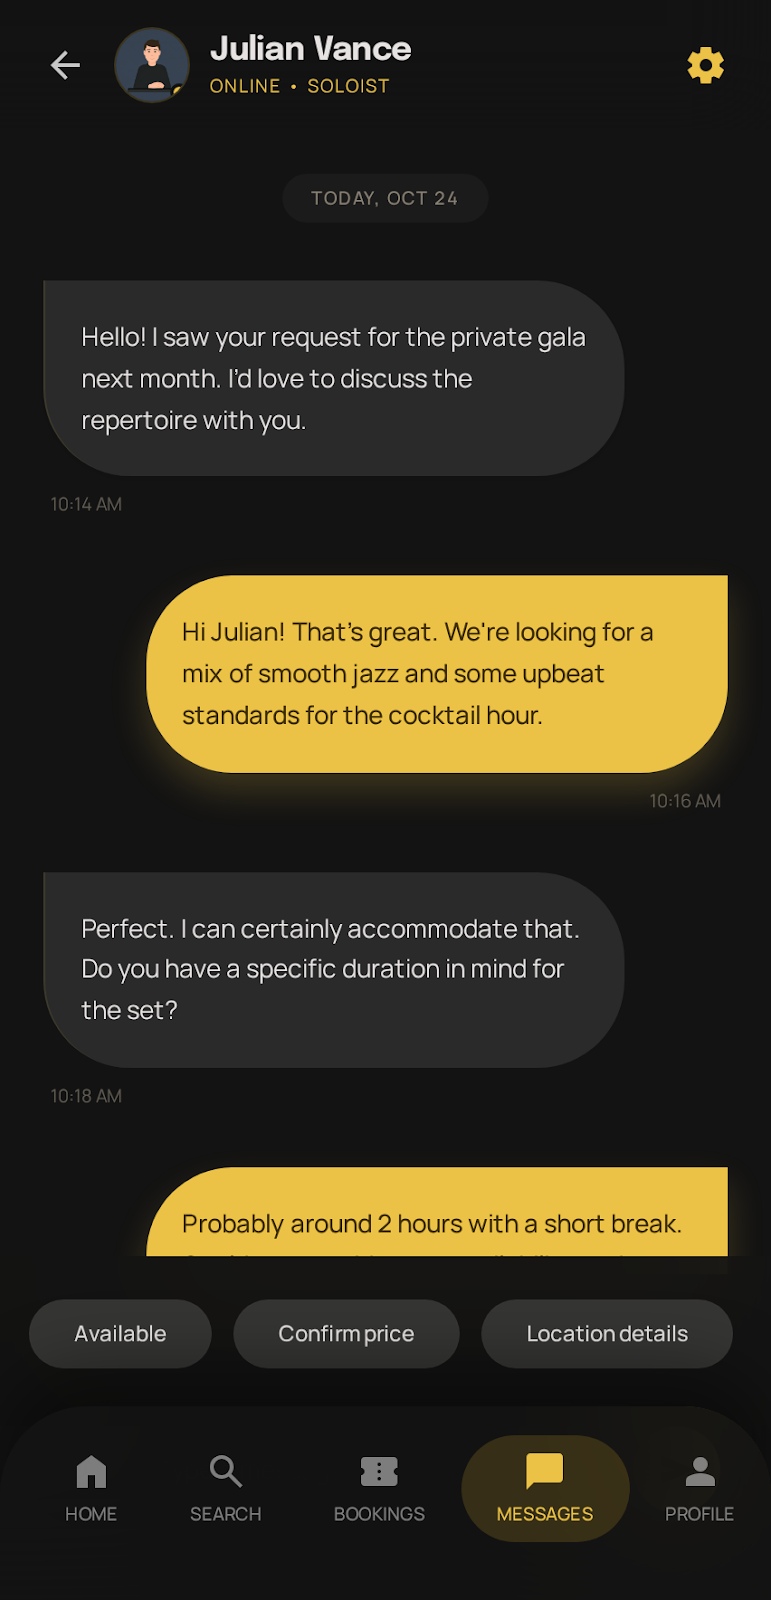
\includegraphics[width=0.44\textwidth]{chat.png}\hfill
    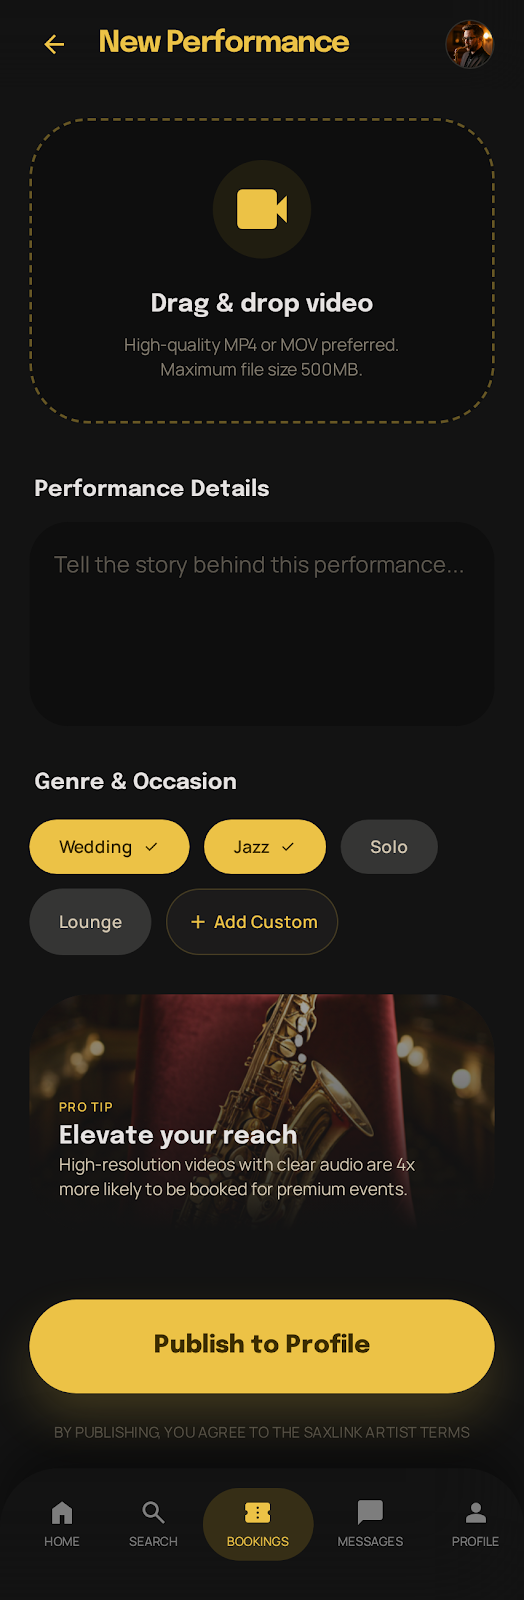
\includegraphics[width=0.44\textwidth]{performance_screen.png}
    \caption{Chat and performance screen}
\end{figure}

\section{Conclusion}
This concept has clear product-market potential when execution stays focused:
\begin{itemize}[leftmargin=1.5em]
    \item Keep the booking flow simple
    \item Build trust through strong performer media and verification
    \item Onboard real performers early and consistently
\end{itemize}

If usability is frictionless, the platform can replace informal referrals with a reliable, scalable talent marketplace.

\end{document}
